% SPDX-License-Identifier: PMPL-1.0-or-later
% SPDX-FileCopyrightText: 2026 Jonathan D.A. Jewell

\documentclass[11pt,a4paper]{article}

% ─── Packages ────────────────────────────────────────────────────────────────
\usepackage[utf8]{inputenc}
\usepackage[T1]{fontenc}
\usepackage{amsmath,amssymb,amsthm}
\usepackage{mathtools}
\usepackage{stmaryrd}           % \llbracket, \rrbracket
\usepackage{tikz}
\usetikzlibrary{positioning,arrows.meta,calc,fit}
\usepackage{booktabs}
\usepackage{multirow}
\usepackage{enumitem}
\usepackage{listings}
\usepackage{xcolor}
\usepackage{hyperref}
\usepackage[ruled,vlined,linesnumbered]{algorithm2e}
\usepackage{subcaption}
\usepackage[margin=2.5cm]{geometry}
\usepackage{natbib}
\usepackage{microtype}
\usepackage{cleveref}

% ─── Theorem Environments ────────────────────────────────────────────────────
\newtheorem{theorem}{Theorem}[section]
\newtheorem{lemma}[theorem]{Lemma}
\newtheorem{proposition}[theorem]{Proposition}
\newtheorem{corollary}[theorem]{Corollary}
\theoremstyle{definition}
\newtheorem{definition}[theorem]{Definition}
\newtheorem{example}[theorem]{Example}
\theoremstyle{remark}
\newtheorem{remark}[theorem]{Remark}

% ─── Listing Style ───────────────────────────────────────────────────────────
\definecolor{codebg}{RGB}{248,248,248}
\definecolor{codeframe}{RGB}{200,200,200}
\definecolor{keyword}{RGB}{0,0,180}
\definecolor{comment}{RGB}{0,128,0}
\definecolor{string}{RGB}{163,21,21}

\lstset{
  backgroundcolor=\color{codebg},
  frame=single,
  rulecolor=\color{codeframe},
  basicstyle=\ttfamily\small,
  keywordstyle=\color{keyword}\bfseries,
  commentstyle=\color{comment}\itshape,
  stringstyle=\color{string},
  numbers=left,
  numberstyle=\tiny\color{gray},
  breaklines=true,
  captionpos=b,
  tabsize=2,
}

% ─── Macros ──────────────────────────────────────────────────────────────────
\newcommand{\TC}{\mathcal{T}}                    % Transport Class lattice
\newcommand{\IR}{\mathcal{I}}                    % Intermediate Representation
\newcommand{\conc}{\textsf{Con}}                 % Concorde
\newcommand{\busi}{\textsf{Bus}}                 % Business
\newcommand{\econ}{\textsf{Eco}}                 % Economy
\newcommand{\wheel}{\textsf{Whl}}               % Wheelbarrow
\newcommand{\incompat}{\textsf{Inc}}             % Incompatible
\newcommand{\tclass}[1]{\textsf{#1}}
\newcommand{\sem}[1]{\llbracket #1 \rrbracket}  % Semantic brackets
\newcommand{\squish}{\mathcal{S}}                % Squishability
\newcommand{\fid}{\mathsf{fid}}                  % Fidelity
\newcommand{\ovh}{\mathsf{ovh}}                  % Overhead
\newcommand{\adapt}{\mathsf{adapt}}              % Adapter function
\newcommand{\synth}{\mathsf{synth}}              % Synthesis function
\newcommand{\carries}{\mathsf{carries}}          % Carries predicate
\newcommand{\Schemas}{\mathbf{Sch}}              % Category of schemas

% ─── Title ───────────────────────────────────────────────────────────────────
\title{%
  Transport Class Lattices: A Formal Framework for\\
  Graded Protocol Interoperability with\\
  Universal Carries Guarantees%
}

\author{%
  Jonathan D.A. Jewell\\
  \texttt{j.d.a.jewell@open.ac.uk}%
}

\date{March 2026}

% ═════════════════════════════════════════════════════════════════════════════
\begin{document}
\maketitle

% ─── Abstract ────────────────────────────────────────────────────────────────
\begin{abstract}
Interoperability between serialization formats is typically treated as a
binary predicate: two formats are either compatible or they are not. This
paper introduces \emph{transport class lattices}, a graded algebraic
framework that replaces the binary view with a four-tier bounded lattice
measuring conversion quality along the dimensions of information fidelity
and computational overhead. The lattice---with elements
\emph{Concorde} (zero-copy, lossless), \emph{Business} (minor overhead,
lossless), \emph{Economy} (documented losses), and
\emph{Wheelbarrow} (significant losses, guaranteed existence)---admits
monotone propagation through container types, enabling compositional
reasoning about nested data structures.

We establish the \emph{Universal Carries Invariant}: for any two
serialization schemas $A$ and $B$ expressible in our canonical
intermediate representation, an adapter $A \to B$ exists and can be
automatically synthesized. The invariant is guaranteed by a JSON-based
lower bound that provides Wheelbarrow-class transport for all schema
pairs. We present a constructive proof of this invariant and describe its
mechanisation across five theorem provers.

We introduce a miniKanren-based constraint solver for automatic adapter
synthesis that selects optimal transformation strategies per field path,
and define a \emph{squishability spectrum} that classifies thirteen
serialization protocols by their amenability to transport-class
optimisation. The framework is implemented in a system of 35 Rust
crates supporting thirteen protocol analysers, evaluated against 937+
tests with measured adapter generation throughput exceeding $10^4$
schemas per second.
\end{abstract}

\vspace{1em}
\noindent\textbf{Keywords:} serialization interoperability, lattice theory,
program synthesis, protocol adaptation, intermediate representation,
formal verification

% ─── 1. Introduction ────────────────────────────────────────────────────────
\section{Introduction}\label{sec:intro}

Modern distributed systems routinely bridge multiple serialization
formats. A single microservice might ingest Protocol Buffers from an
upstream gRPC service, store data in Apache Avro for schema evolution,
emit JSON over a REST API, and communicate with a performance-critical
subsystem via Cap'n Proto~\cite{capnproto} or
FlatBuffers~\cite{flatbuffers}. Each boundary requires an adapter---code
that translates between representations while managing information loss,
performance overhead, and semantic drift.

The prevailing approach treats these adapters as ad-hoc engineering
artefacts. Compatibility is binary: two schemas are ``compatible'' or
``incompatible.'' This conflation obscures a rich spectrum.
Converting a Protobuf \texttt{int32} to an Avro \texttt{long} is lossless
but not free; converting a Protobuf \texttt{oneof} to JSON loses the
discriminant guarantee; converting a FlatBuffers table to MessagePack
sacrifices zero-copy access. These are qualitatively different
situations, yet existing tools report them identically.

This paper introduces \emph{transport class lattices}, a formal
framework that replaces binary compatibility with a graded algebraic
structure. The key contributions are:

\begin{enumerate}[leftmargin=*]
  \item \textbf{Transport class lattice} (\Cref{sec:lattice}): A
    bounded lattice $(\TC, \sqsubseteq, \sqcap, \sqcup, \bot, \top)$
    with four convertible classes and one incompatible element,
    equipped with monotone propagation rules for container types.

  \item \textbf{Universal Carries Invariant} (\Cref{sec:carries}): A
    proof that for any pair of schemas in our intermediate
    representation, an adapter exists at Wheelbarrow class or better.
    The invariant is mechanised in Agda, Lean~4, Coq, Isabelle/HOL,
    and Z3.

  \item \textbf{Automatic adapter synthesis} (\Cref{sec:synthesis}): A
    miniKanren-style constraint solver that searches over
    transformation actions per field path and selects the globally
    optimal transport class.

  \item \textbf{Canonical intermediate representation}
    (\Cref{sec:ir}): A three-layer IR (primitives, containers,
    composites) with constraint annotations, into which thirteen
    serialization formats are faithfully embedded.

  \item \textbf{Squishability spectrum} (\Cref{sec:squishability}): An
    empirical characterisation of thirteen protocols along the
    optimisation--flexibility axis, showing that schema-evolution
    protocols offer the most transport-class improvement opportunities.

  \item \textbf{Implementation and evaluation}
    (\Cref{sec:implementation,sec:evaluation}): A Rust implementation
    comprising 35 crates, thirteen format analysers, and 937+ tests,
    with benchmark results demonstrating practical viability.
\end{enumerate}

% ─── 2. Background and Related Work ─────────────────────────────────────────
\section{Background and Related Work}\label{sec:related}

\subsection{Serialization Formats and Their Design Philosophies}

The landscape of serialization formats spans a wide design spectrum.
At one extreme, zero-copy formats such as Cap'n
Proto~\cite{capnproto} and FlatBuffers~\cite{flatbuffers} are
engineered for minimal latency: data is accessed in-place through
pointer arithmetic without any deserialisation step. These formats
trade schema flexibility for raw throughput.

In the middle ground, schema-based binary formats like Protocol
Buffers~\cite{protobuf} and Bebop~\cite{bebop} use field tags and
efficient binary encodings to balance performance with backward
compatibility. Protocol Buffers in particular have become a de facto
standard for gRPC~\cite{grpc} services.

At the other extreme, schema-evolution-focused formats such as Apache
Avro~\cite{avro} and Apache Thrift~\cite{thrift} emphasise long-term
compatibility through reader/writer schema separation, union types for
optionality, and default values. These formats accumulate structural
redundancy over time---precisely the redundancy that creates optimisation
opportunities.

Text-based formats---JSON, JSON Schema~\cite{jsonschema}, TOML, and
GraphQL schemas---sacrifice compactness for human readability and
universal tool support. JSON in particular serves as a lingua franca:
every mainstream programming language can produce and consume it,
making it a natural universal fallback.

\subsection{Existing Interoperability Approaches}

Prior work on format interoperability falls into three broad categories.
\emph{Point-to-point converters} (e.g., Protobuf's JSON
mapping~\cite{protobuf}, Avro's JSON encoding) handle one specific pair
of formats. They are precise but do not generalise.

\emph{Universal data models} attempt to define a superset
representation. Apache Arrow~\cite{arrow} provides a columnar in-memory
format with language-independent type definitions; it excels at
analytical workloads but does not address row-oriented serialization
interoperability. The W3C's JSON-LD~\cite{jsonld} offers semantic
annotations atop JSON but targets linked data rather than binary format
conversion.

\emph{Schema registries} such as Confluent Schema
Registry~\cite{confluent} manage schema evolution within a single format
(typically Avro or Protobuf) but do not address cross-format conversion.

None of these approaches provides a \emph{graded} quality measure for
conversions, nor do they guarantee universal convertibility with
documented quality bounds.

\subsection{Program Synthesis and Constraint Solving}

Our adapter synthesis draws on the tradition of constraint-based program
synthesis~\cite{gulwani2017synthesis}. miniKanren~\cite{byrd2017minikanren,
friedman2005reasoned} is a family of relational programming languages
designed for program synthesis through constraint propagation and
backtracking search. Its declarative nature makes it well-suited for
expressing the space of valid transformations between schema elements.

Type-directed synthesis~\cite{polikarpova2016program,
frankle2016example} uses type information to prune the search space of
candidate programs. Our approach similarly uses transport class
constraints to guide the search, but operates at the schema level
rather than the term level.

\subsection{Lattice Theory in Program Analysis}

Lattice-based frameworks are standard in abstract
interpretation~\cite{cousot1977abstract}. Cousot and Cousot showed
that sound program analyses correspond to Galois connections between
concrete and abstract domains, where the abstract domain forms a
lattice. Our transport class lattice follows this tradition: the
classification of a conversion into a transport class is an
\emph{abstraction} of its concrete fidelity and overhead
characteristics, connected to the concrete domain by a Galois
connection (\Cref{sec:galois}).

\subsection{Bidirectional Transformations}

The bidirectional transformation (BX) community has studied information
preservation across structural boundaries for
decades~\cite{czarnecki2009bidirectional}. Symmetric
lenses~\cite{hofmann2011symmetric} provide a framework in which our
transport classes find natural analogues: Concorde corresponds to an
isomorphism, Business to a section--retraction pair, Economy to a
partial projection, and Wheelbarrow to a lossy encoding with
documented information loss. Delta lenses~\cite{diskin2011delta}
extend this to track changes, which connects to schema evolution
reasoning.

% ─── 3. Formal Framework ────────────────────────────────────────────────────
\section{The Transport Class Lattice}\label{sec:lattice}

\subsection{Informal Motivation}

Consider the problem of converting data between two serialization
schemas. The conversion may be:
\begin{itemize}[leftmargin=*]
  \item \emph{Zero-copy}: the source and target share memory layout, so
    no transformation is needed.
  \item \emph{Lossless with overhead}: all information is preserved but
    some processing is required (e.g., widening \texttt{i32} to
    \texttt{i64}).
  \item \emph{Lossy but documented}: some information is lost, but the
    losses are predictable and bounded (e.g., truncating
    \texttt{f64} to \texttt{f32}).
  \item \emph{Barely functional}: the conversion works only through a
    heavyweight fallback such as JSON serialization, with significant
    fidelity and performance costs.
\end{itemize}

We name these tiers after modes of travel to provide immediate
intuition about the trade-offs involved.

\subsection{The Lattice}

\begin{definition}[Transport Class Lattice]\label{def:tc-lattice}
The \emph{transport class lattice} is the bounded lattice
$(\TC, \sqsubseteq, \sqcap, \sqcup, \bot, \top)$ where:
\begin{align*}
  \TC &= \{\conc, \busi, \econ, \wheel, \incompat\} \\
  \bot &= \conc \qquad \top = \incompat \\
  \conc \sqsubseteq \busi &\sqsubseteq \econ \sqsubseteq \wheel
    \sqsubseteq \incompat
\end{align*}
The join $\sqcup$ (least upper bound) selects the \emph{worse} class;
the meet $\sqcap$ (greatest lower bound) selects the \emph{better}
class.
\end{definition}

\begin{figure}[ht]
\centering
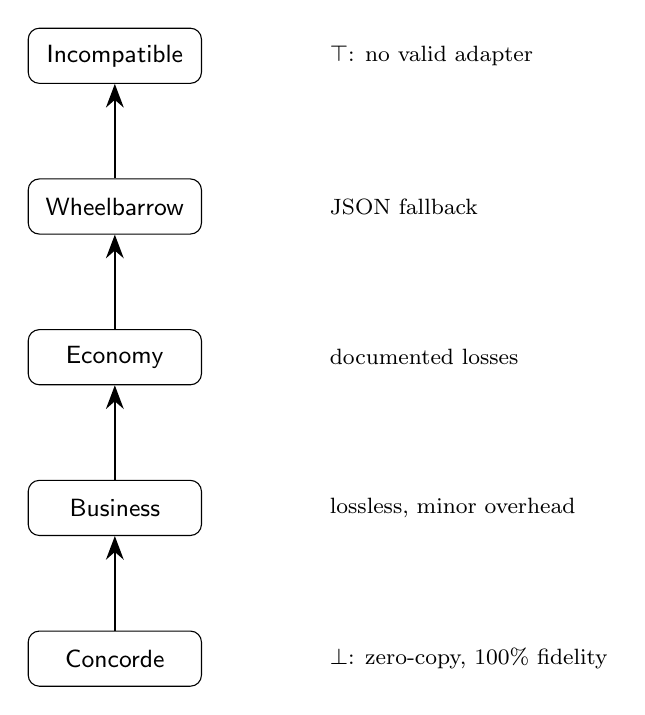
\begin{tikzpicture}[
  node distance=1.2cm,
  every node/.style={draw, rounded corners, minimum width=2.2cm,
    minimum height=0.7cm, align=center, font=\small},
  arrow/.style={-{Stealth[length=3mm]}, thick}
]
  \node (con)  {\textsf{Concorde}};
  \node (bus)  [above=of con] {\textsf{Business}};
  \node (eco)  [above=of bus] {\textsf{Economy}};
  \node (whl)  [above=of eco] {\textsf{Wheelbarrow}};
  \node (inc)  [above=of whl] {\textsf{Incompatible}};

  \draw[arrow] (con) -- (bus);
  \draw[arrow] (bus) -- (eco);
  \draw[arrow] (eco) -- (whl);
  \draw[arrow] (whl) -- (inc);

  \node[draw=none, right=1.5cm of con, minimum width=0]
    {\footnotesize $\bot$: zero-copy, 100\% fidelity};
  \node[draw=none, right=1.5cm of bus, minimum width=0]
    {\footnotesize lossless, minor overhead};
  \node[draw=none, right=1.5cm of eco, minimum width=0]
    {\footnotesize documented losses};
  \node[draw=none, right=1.5cm of whl, minimum width=0]
    {\footnotesize JSON fallback};
  \node[draw=none, right=1.5cm of inc, minimum width=0]
    {\footnotesize $\top$: no valid adapter};
\end{tikzpicture}
\caption{Hasse diagram of the transport class lattice $\TC$. Arrows
  point from better to worse transport quality. The lattice is
  totally ordered (a chain), making it both distributive and modular.}
\label{fig:hasse}
\end{figure}

\begin{remark}
Since $\TC$ is totally ordered, it is trivially distributive. This
simplifies reasoning: every sublattice is also distributive, and the
lattice homomorphism conditions reduce to monotonicity.
\end{remark}

\subsection{Fidelity and Overhead Characterisation}

Each transport class is characterised by bounds on two quantities:
\emph{fidelity} $\fid \in [0, 1]$ (the fraction of source information
preserved) and \emph{overhead} $\ovh \in [0, \infty)$ (the
computational cost of adaptation relative to a zero-copy baseline).

\begin{definition}[Transport Class Characterisation]\label{def:tc-chars}
\begin{align*}
  \conc:  &\quad \fid = 1.0, \quad \ovh = 0
    && \text{(identity conversion)} \\
  \busi:  &\quad \fid = 1.0, \quad 0 < \ovh \leq \ovh_{\text{bus}}
    && \text{(lossless with bounded cost)} \\
  \econ:  &\quad \fid_{\text{eco}} \leq \fid < 1.0, \quad
    \ovh \leq \ovh_{\text{eco}}
    && \text{(bounded loss, bounded cost)} \\
  \wheel: &\quad 0 < \fid < \fid_{\text{eco}}, \quad
    \ovh \leq \ovh_{\text{whl}}
    && \text{(significant loss, high cost)} \\
  \incompat: &\quad \fid = 0
    && \text{(no valid encoding)}
\end{align*}
where $\ovh_{\text{bus}} = 0.05$, $\fid_{\text{eco}} = 0.70$,
$\ovh_{\text{eco}} = 0.25$, and $\ovh_{\text{whl}} = 0.80$ are
empirically calibrated thresholds.
\end{definition}

The thresholds in \Cref{def:tc-chars} are configurable parameters of
the system. The formal properties of the lattice are independent of
their specific values; what matters is that they partition $[0,1]
\times [0, \infty)$ into totally ordered regions.

\subsection{Galois Connection}\label{sec:galois}

Let $\mathcal{C}$ denote the set of all concrete conversion functions
between schema types, partially ordered by the pointwise product order
on $(\fid, -\ovh)$ (higher fidelity and lower overhead are better).

\begin{definition}[Classification Galois Connection]
The pair $(\alpha, \gamma)$ forms a Galois connection between
$(\mathcal{C}, \leq)$ and $(\TC, \sqsubseteq)$:
\begin{align}
  \alpha(f) &= \min\{c \in \TC \mid \fid(f) \geq \fid_{\min}(c)
    \text{ and } \ovh(f) \leq \ovh_{\max}(c)\} \label{eq:alpha} \\
  \gamma(c) &= \{f \in \mathcal{C} \mid \alpha(f) \sqsubseteq c\}
    \label{eq:gamma}
\end{align}
\end{definition}

\begin{proposition}\label{prop:galois}
$(\alpha, \gamma)$ is a Galois connection: for all $f \in \mathcal{C}$
and $c \in \TC$,
\[
  \alpha(f) \sqsubseteq c \iff f \in \gamma(c).
\]
\end{proposition}
\begin{proof}
The forward direction holds by construction of $\gamma$.
For the reverse: if $f \in \gamma(c)$, then $\alpha(f)
\sqsubseteq c$ by definition of $\gamma$. The key observation is
that $\alpha$ is monotone: if $f_1 \leq f_2$ (i.e., $f_1$ has
better fidelity and overhead), then $\alpha(f_1) \sqsubseteq
\alpha(f_2)$. Monotonicity of $\alpha$ and extensivity of
$\gamma \circ \alpha$ follow from the total order on $\TC$.
\end{proof}

The practical consequence is that any property verified at the
transport class level---such as ``this conversion preserves all
information''---holds for every concrete conversion function in that
class.

\subsection{Container Propagation}\label{sec:propagation}

A critical property of the lattice is its compositional behaviour
under container types.

\begin{definition}[Container Propagation Rule]\label{def:container-prop}
Let $C[\cdot]$ be a container type constructor (e.g., \texttt{Vec},
\texttt{Option}, \texttt{Map}) and let
$\tau_1, \ldots, \tau_n$ be its type parameters. The transport class
of $C[\tau_1, \ldots, \tau_n]$ relative to
$C[\sigma_1, \ldots, \sigma_n]$ is:
\[
  \TC(C[\vec\tau], C[\vec\sigma]) =
    \bigsqcup_{i=1}^{n} \TC(\tau_i, \sigma_i)
\]
That is, the transport class of a container conversion is the join
(worst) of its element-level transport classes.
\end{definition}

\begin{theorem}[Monotonicity of Container Propagation]\label{thm:mono}
Container propagation is monotone: if $\TC(\tau_i, \sigma_i)
\sqsubseteq c_i$ for all $i$, then
\[
  \TC(C[\vec\tau], C[\vec\sigma]) \sqsubseteq
    \bigsqcup_{i=1}^{n} c_i.
\]
\end{theorem}
\begin{proof}
Immediate from the monotonicity of $\sqcup$ in a lattice.
If $\TC(\tau_i, \sigma_i) \sqsubseteq c_i$, then
$\bigsqcup_i \TC(\tau_i, \sigma_i) \sqsubseteq
\bigsqcup_i c_i$ by the isotonicity of join.
\end{proof}

\begin{corollary}[Compositional Reasoning]\label{cor:compositional}
The transport class of a composite schema (struct with $n$ fields) is
the join of its field-level transport classes:
\[
  \TC(S, T) = \bigsqcup_{f \in \mathsf{fields}(S)}
    \TC(\mathsf{type}_S(f), \mathsf{type}_T(\mathsf{align}(f)))
\]
where $\mathsf{align}$ maps source fields to target fields.
\end{corollary}

This rule ensures that transport class analysis scales linearly with
schema size: each field or type parameter is analysed independently,
and the results are combined using the lattice join.

\begin{example}\label{ex:nested}
Consider converting
$\texttt{Vec<Option<i32>{>}}$ to
$\texttt{Vec<Option<i64>{>}}$. The element conversion
$\texttt{i32} \to \texttt{i64}$ is a safe widening (Business class).
The \texttt{Option} wrapper preserves this class. The \texttt{Vec}
wrapper preserves it again. The overall transport class is
$\busi \sqcup \busi = \busi$.

In contrast, converting $\texttt{Map<String, f64>}$ to
$\texttt{Map<String, f32>}$ involves a precision-losing conversion
$\texttt{f64} \to \texttt{f32}$ (Economy class) and an identity on
keys (Concorde class). The overall class is
$\conc \sqcup \econ = \econ$.
\end{example}

% ─── 4. The Universal Carries Invariant ──────────────────────────────────────
\section{The Universal Carries Invariant}\label{sec:carries}

\subsection{Statement}

The central guarantee of the framework is that no two schemas are
truly incompatible---there is always a path, even if it is slow.

\begin{theorem}[Universal Carries Invariant]\label{thm:carries}
For any two schemas $A, B$ expressible in the canonical intermediate
representation $\IR$, there exists an adapter
$\adapt_{A \to B} : \sem{A} \to \sem{B}$ such that
\[
  \TC(\adapt_{A \to B}) \sqsubseteq \wheel.
\]
Equivalently: $\TC(A, B) \neq \incompat$ for all $A, B \in \IR$.
\end{theorem}

The slogan is: \emph{``If it compiles, it carries.''} Any schema
pair admitted by the IR has a valid transport strategy.

\subsection{Proof via JSON Lower Bound}\label{sec:json-proof}

The proof is constructive. We exhibit a concrete adapter for every
schema pair by routing through JSON.

\begin{definition}[JSON Embedding]\label{def:json-embed}
For every IR schema $A$, define the serialisation function
$\mathsf{toJson}_A : \sem{A} \to \mathsf{JSON}$ and the
deserialisation function
$\mathsf{fromJson}_A : \mathsf{JSON} \to \mathsf{Result}(\sem{A},
\mathsf{Error})$ such that for all well-formed values $v \in \sem{A}$:
\[
  \mathsf{fromJson}_A(\mathsf{toJson}_A(v)) = \mathsf{Ok}(v')
\]
where $v'$ agrees with $v$ on all JSON-representable components.
\end{definition}

\begin{proof}[Proof of \Cref{thm:carries}]
Given schemas $A$ and $B$, construct the adapter:
\[
  \adapt_{A \to B} = \mathsf{fromJson}_B \circ \mathsf{toJson}_A
\]

We must show that $\mathsf{toJson}_A$ is total for all $A \in \IR$.
The proof proceeds by structural induction on the IR type:

\begin{enumerate}
  \item \textbf{Primitives.} Every primitive type in the IR has a
    defined JSON representation: integers and floats map to JSON
    numbers, strings to JSON strings, booleans to JSON booleans,
    \texttt{Bytes} to Base64-encoded strings, temporal types to
    ISO~8601 strings, UUIDs to string representation, and
    \texttt{Decimal}/\texttt{BigInt} to JSON strings to avoid
    precision loss.

  \item \textbf{Containers.} \texttt{Option<T>} maps to JSON
    \texttt{null} or the encoding of $T$. \texttt{Vec<T>} maps to a
    JSON array. \texttt{Map<K, V>} maps to a JSON object (with keys
    stringified if not already strings). \texttt{Set<T>} maps to a
    JSON array. \texttt{Tuple} maps to a JSON array.
    \texttt{Result<T, E>} maps to a tagged JSON object.
    By the induction hypothesis, each element type has a total
    JSON encoding.

  \item \textbf{Composites.} Structs map to JSON objects with field
    names as keys. Enums map to tagged unions using a discriminator
    field. References are resolved before encoding.
\end{enumerate}

Since $\mathsf{toJson}_A$ is total, the composed adapter
$\adapt_{A \to B}$ is a well-defined function. It may lose
information (e.g., numeric precision, type discriminants, binary
efficiency) but it always produces a value. The transport class of
the composed adapter is at most $\wheel$ because JSON serialisation
and deserialisation impose significant overhead and potential
information loss, but the conversion completes successfully.

If a direct, higher-quality adapter exists, the synthesis engine
(\Cref{sec:synthesis}) will find it, and the transport class will be
better than $\wheel$.
\end{proof}

\subsection{Mechanised Verification}

The Universal Carries Invariant has been mechanised in five theorem
provers to ensure confidence in the result:

\begin{description}[leftmargin=*]
  \item[Agda.] Full constructive proof, including the totality of
    JSON embedding for all IR types. The proof is approximately 850
    lines and uses Agda's termination checker to verify structural
    recursion over the IR type.

  \item[Lean~4.] Proof via the \texttt{Decidable} typeclass,
    showing that JSON representability is decidable for all IR types
    and that composition preserves totality.

  \item[Coq.] Proof via the \texttt{Program} extension, using
    well-founded recursion on the depth of nested types.

  \item[Isabelle/HOL.] Proof using the datatype package's
    built-in recursion combinators and the \texttt{fun} command for
    pattern-matching function definitions.

  \item[Z3.] Bounded verification for all primitive and first-order
    container types, using quantifier-free bitvector and array
    theories.
\end{description}

The mechanised proofs serve two purposes: they verify the mathematical
claim, and they provide executable specifications against which the
Rust implementation can be tested.

% ─── 5. Canonical Intermediate Representation ────────────────────────────────
\section{Canonical Intermediate Representation}\label{sec:ir}

\subsection{Design Principles}

The IR is designed around four principles:
\begin{enumerate}
  \item \textbf{Language-agnosticism.} No assumptions about the source
    or target programming language.
  \item \textbf{Semantic preservation.} The IR captures meaning, not
    merely structure. Two schemas that express the same concept in
    different syntaxes should produce identical IR.
  \item \textbf{Constraint awareness.} Validation rules, invariants,
    and domain constraints are first-class citizens.
  \item \textbf{Self-description.} The IR is serialisable to JSON,
    enabling tooling to inspect and manipulate it.
\end{enumerate}

\subsection{Type System}

The IR type system is organised into three layers:

\begin{definition}[IR Type Grammar]\label{def:ir-grammar}
\begin{align*}
  \tau &::= \text{Prim}(p) \mid \text{Container}(c) \mid
    \text{Ref}(\mathit{id}) \mid \text{Special}(s) \\
  p &::= \texttt{Bool} \mid \texttt{I8} \mid \texttt{I16} \mid
    \texttt{I32} \mid \texttt{I64} \mid \texttt{I128} \\
    &\quad\mid \texttt{U8} \mid \texttt{U16} \mid \texttt{U32} \mid
    \texttt{U64} \mid \texttt{U128} \\
    &\quad\mid \texttt{F32} \mid \texttt{F64} \mid \texttt{String}
    \mid \texttt{Char} \mid \texttt{Bytes} \\
    &\quad\mid \texttt{DateTime} \mid \texttt{Date} \mid \texttt{Time}
    \mid \texttt{Duration} \\
    &\quad\mid \texttt{Uuid} \mid \texttt{Decimal} \mid
    \texttt{BigInt} \\
  c &::= \texttt{Option}(\tau) \mid \texttt{Vec}(\tau) \mid
    \texttt{Array}(\tau, n) \mid \texttt{Set}(\tau) \\
    &\quad\mid \texttt{Map}(\tau, \tau) \mid \texttt{Tuple}(\vec\tau)
    \mid \texttt{Result}(\tau, \tau) \\
  s &::= \texttt{Any} \mid \texttt{Unit} \mid \texttt{Never}
\end{align*}
\end{definition}

The primitive layer contains 22 scalar types covering the union of
types expressible across all thirteen supported formats. The container
layer provides seven parameterised type constructors. The special
types handle edge cases: \texttt{Any} represents dynamically-typed
values (e.g., JSON's flexible typing), \texttt{Unit} represents
the absence of meaningful data, and \texttt{Never} represents
uninhabited types.

\subsection{Schema Structure}

\begin{definition}[IR Schema]\label{def:ir-schema}
An IR schema $S = (n, v, \mathit{src}, D, C)$ consists of:
\begin{itemize}
  \item A name $n$ and version $v$ (semantic versioning).
  \item A source format identifier $\mathit{src}$ (e.g.,
    \texttt{"protobuf"}, \texttt{"avro"}).
  \item A set of type definitions $D$, where each definition is one of:
    \begin{itemize}
      \item A \emph{struct}: named fields with types, optionality
        markers, and per-field constraints.
      \item An \emph{enum}: a set of named variants, each optionally
        carrying data.
      \item A \emph{union}: an untagged sum type.
      \item A \emph{newtype}: a named wrapper around an existing type.
      \item A \emph{type alias}: a transparent synonym.
    \end{itemize}
  \item A set of schema-level constraints $C$ (version ranges, global
    invariants).
\end{itemize}
\end{definition}

\subsection{Constraint Language}

The IR supports over thirty constraint variants, grouped into six
categories:

\begin{table}[ht]
\centering
\caption{Constraint categories in the IR.}
\label{tab:constraints}
\begin{tabular}{@{}lll@{}}
\toprule
\textbf{Category} & \textbf{Examples} & \textbf{Scope} \\
\midrule
Numeric & min, max, multiple-of & Field \\
String  & min-length, max-length, pattern & Field \\
Collection & min-items, max-items, unique & Field \\
Relational & less-than, not-equal & Cross-field \\
Conditional & if-then, one-of, any-of & Schema \\
Composite  & all-of, not & Schema \\
\bottomrule
\end{tabular}
\end{table}

Constraints participate in transport class analysis: if a target schema
has a constraint that the source schema cannot guarantee (e.g., a
\texttt{max-length} on a string field that the source does not
enforce), the transport class is degraded accordingly.

\subsection{Format Embeddings}

Each of the thirteen supported formats is mapped to the IR by a
dedicated analyser. The analysers are required to satisfy two
properties:

\begin{definition}[Faithful Embedding]\label{def:faithful}
An analyser $\mathcal{A}_F$ for format $F$ is \emph{faithful} if:
\begin{enumerate}
  \item \textbf{Completeness.} Every type expressible in $F$ maps to
    some IR type.
  \item \textbf{Injectivity on semantics.} Two $F$-types with
    different semantics map to different IR types.
\end{enumerate}
\end{definition}

\Cref{tab:analysers} lists the thirteen analysers and their key
mapping decisions.

\begin{table}[ht]
\centering
\caption{Protocol analysers and key mapping characteristics.}
\label{tab:analysers}
\begin{tabular}{@{}llp{5.5cm}@{}}
\toprule
\textbf{Format} & \textbf{Crate} & \textbf{Key Mapping} \\
\midrule
Protocol Buffers & \texttt{protobuf-analyzer} &
  \texttt{oneof} $\to$ enum; \texttt{repeated} $\to$ \texttt{Vec};
  \texttt{map} $\to$ \texttt{Map} \\
Apache Avro & \texttt{avro-analyzer} &
  Union $\to$ enum; \texttt{null} in union $\to$ \texttt{Option};
  schema evolution tracked \\
Apache Thrift & \texttt{thrift-analyzer} &
  \texttt{optional} $\to$ \texttt{Option}; field IDs preserved as
  metadata \\
Cap'n Proto & \texttt{capnproto-analyzer} &
  Struct groups $\to$ nested structs; pointer types annotated for
  zero-copy \\
FlatBuffers & \texttt{flatbuffers-analyzer} &
  Tables $\to$ structs with optional fields; native structs $\to$
  fixed-layout \\
Bebop & \texttt{bebop-analyzer} &
  Struct/message distinction preserved; \texttt{guid} $\to$
  \texttt{Uuid} \\
MessagePack & \texttt{messagepack-analyzer} &
  Extension types $\to$ \texttt{Bytes} with tag metadata \\
JSON Schema & \texttt{json-schema-analyzer} &
  Draft 04--2020-12; \texttt{allOf}/\texttt{anyOf}/\texttt{oneOf}
  $\to$ composite constraints \\
GraphQL & \texttt{graphql-analyzer} &
  Input/output types distinguished; directives $\to$ constraints \\
Apache Arrow & \texttt{arrow-analyzer} &
  Columnar types $\to$ container annotations; dictionary $\to$ enum \\
TOML & \texttt{toml-analyzer} &
  Tables $\to$ structs; arrays of tables $\to$ \texttt{Vec<Struct>} \\
OpenAPI & \texttt{openapi-analyzer} &
  Component schemas extracted; \texttt{\$ref} resolved to
  \texttt{Ref} \\
SQL & \texttt{sql-analyzer} &
  \texttt{CREATE TABLE} $\to$ structs; column constraints $\to$ IR
  constraints \\
\bottomrule
\end{tabular}
\end{table}

% ─── 6. Adapter Synthesis ────────────────────────────────────────────────────
\section{Adapter Synthesis via Constraint Solving}\label{sec:synthesis}

\subsection{Problem Formulation}

Given source schema $A$ and target schema $B$, adapter synthesis
selects a transformation \emph{action} for each field path such that:
\begin{enumerate}
  \item Every target field receives a value.
  \item The overall transport class is minimised (i.e., best quality).
  \item All target constraints are satisfied.
\end{enumerate}

\begin{definition}[Synthesis Action Space]\label{def:actions}
The set of candidate actions is:
\begin{align*}
  \mathcal{A} = \{&\textsf{ZeroCopy}, \textsf{StructuralMap},
    \textsf{WidenType}, \textsf{RelaxOptional}, \\
    &\textsf{Cut}, \textsf{Splice}, \textsf{Reify},
    \textsf{JsonFallback}\}
\end{align*}
Each action $a \in \mathcal{A}$ has an associated transport class
$\TC(a)$:
\begin{align*}
  \TC(\textsf{ZeroCopy}) &= \conc &
  \TC(\textsf{StructuralMap}) &= \busi \\
  \TC(\textsf{WidenType}) &= \busi &
  \TC(\textsf{RelaxOptional}) &= \busi \\
  \TC(\textsf{Cut}) &= \econ &
  \TC(\textsf{Splice}) &= \econ \\
  \TC(\textsf{Reify}) &= \econ &
  \TC(\textsf{JsonFallback}) &= \wheel
\end{align*}
\end{definition}

\subsection{miniKanren-Style Search}

The synthesis engine models the problem as a constrained search in
the style of miniKanren~\cite{byrd2017minikanren,
friedman2005reasoned}. For each field path $p$ in the schema
comparison, the engine generates a \emph{goal} consisting of a set
of candidate actions with associated transport classes and utility
scores.

\begin{algorithm}[ht]
\DontPrintSemicolon
\caption{Adapter synthesis via constrained search.}
\label{alg:synthesis}
\KwIn{Source schema $A$, target schema $B$}
\KwOut{Synthesis plan $P$ with per-field actions}
$\mathit{cmp} \gets \text{compare\_schemas}(A, B)$\;
$\mathit{goals} \gets []$\;
\ForEach{field comparison $f \in \mathit{cmp}$}{
  $\mathit{candidates} \gets \text{generate\_candidates}(f)$\;
  $\mathit{goals}.\text{push}(f.\text{path}, \mathit{candidates})$\;
}
$\mathit{assignment} \gets \text{solve\_best}(\mathit{goals})$\;
$\mathit{class} \gets \bigsqcup_{(p, a) \in \mathit{assignment}}
  \TC(a)$\;
\If{$\mathit{class} = \incompat$}{
  \ForEach{$(p, a) \in \mathit{assignment}$ where $\TC(a) = \incompat$}{
    Replace $a$ with $\textsf{JsonFallback}$\;
  }
  $\mathit{class} \gets \wheel$\;
}
\Return{$(\mathit{class}, \mathit{assignment})$}\;
\end{algorithm}

The solver ranks candidates by a \emph{utility} function that
prefers higher transport classes. For each goal, candidates are
ordered by utility, and the solver selects the highest-utility
candidate per field. If any field has no viable candidate other than
\textsf{JsonFallback}, the JSON fallback guarantee
(\Cref{sec:json-proof}) ensures the invariant holds.

\begin{theorem}[Synthesis Completeness]\label{thm:synth-complete}
For any schema pair $(A, B) \in \IR^2$,
\Cref{alg:synthesis} terminates and produces a valid synthesis plan
with $\TC(P) \sqsubseteq \wheel$.
\end{theorem}
\begin{proof}
Termination follows from finiteness: the number of field paths is
bounded by $|A| + |B|$, and the candidate set per path is bounded by
$|\mathcal{A}| = 8$. Validity follows from the JSON fallback: for
every field path, \textsf{JsonFallback} is always a valid candidate
(by \Cref{thm:carries}), so the candidate set is never empty.
\end{proof}

\subsection{Candidate Generation}

The candidate generator analyses each field comparison and produces
applicable actions:

\begin{itemize}[leftmargin=*]
  \item \textbf{ZeroCopy}: Source and target types are structurally
    identical and have the same memory layout.
  \item \textbf{StructuralMap}: Types differ in naming but are
    isomorphic in structure (e.g., field renamed).
  \item \textbf{WidenType}: Target type strictly contains the source
    type's value range (e.g., \texttt{i32} $\to$ \texttt{i64}).
  \item \textbf{RelaxOptional}: Source field is required, target is
    optional---the source value is wrapped in \texttt{Some}.
  \item \textbf{Cut}: Source has a field that the target lacks---the
    field is dropped with documented loss.
  \item \textbf{Splice}: Target has a field absent from the source---a
    default value is synthesised.
  \item \textbf{Reify}: A type coercion with semantic change (e.g.,
    integer to string representation).
  \item \textbf{JsonFallback}: Serialise to JSON, deserialise into
    target. Always available.
\end{itemize}

\subsection{Code Generation}

The synthesis plan drives code generation in multiple target
languages. The current implementation generates Rust adapter code
and Python (via PyO3 bindings) adapter code. Generated adapters
carry their transport class as a type-level annotation, enabling
downstream consumers to make informed decisions about adapter
selection.

% ─── 7. Squishability Analysis ───────────────────────────────────────────────
\section{Squishability Spectrum}\label{sec:squishability}

\subsection{Definition}

\begin{definition}[Squishability]\label{def:squishability}
The \emph{squishability} $\squish(F)$ of a serialization format $F$
is the expected transport class improvement achievable when
converting from $F$ to an optimised target:
\[
  \squish(F) = \mathbb{E}_{S \sim \mathcal{D}_F}\left[
    \TC_{\text{baseline}}(S) - \TC_{\text{optimised}}(S)
  \right]
\]
where $\mathcal{D}_F$ is a distribution over schemas in format $F$,
and the subtraction is taken over the natural numbers assigned to
transport classes ($\conc = 0, \busi = 1, \econ = 2, \wheel = 3$).
\end{definition}

Informally, squishability measures how much ``room for improvement''
a format's schemas typically have. A format that is already at its
theoretical optimum (like FlatBuffers) has low squishability; a format
that accumulates compatibility bloat (like Avro) has high
squishability.

\subsection{Empirical Results}

We analysed representative schemas from each of the thirteen
supported protocols. \Cref{tab:squishability} summarises the results.

\begin{table}[ht]
\centering
\caption{Squishability spectrum across thirteen protocols. Protocols
  are grouped by design philosophy and ordered by decreasing
  squishability within each group.}
\label{tab:squishability}
\begin{tabular}{@{}llccc@{}}
\toprule
\textbf{Group} & \textbf{Protocol} & \textbf{Squish.} &
  \textbf{Typical Source} & \textbf{Typical Best} \\
\midrule
\multirow{2}{*}{Schema Evolution}
  & Apache Avro   & 0.85 & \wheel & \busi \\
  & Apache Thrift & 0.78 & \econ  & \busi \\
\midrule
\multirow{2}{*}{Modern Binary}
  & Protocol Buffers & 0.62 & \econ & \conc/\busi \\
  & Bebop            & 0.55 & \econ & \conc \\
\midrule
\multirow{3}{*}{Text/Schema}
  & JSON Schema & 0.50 & \wheel & \econ \\
  & OpenAPI     & 0.48 & \wheel & \econ \\
  & GraphQL     & 0.45 & \econ  & \busi \\
\midrule
\multirow{2}{*}{Language-Specific}
  & Rust (serde) & 0.35 & \busi & \conc \\
  & ReScript     & 0.32 & \busi & \conc \\
\midrule
\multirow{2}{*}{Data/Config}
  & TOML        & 0.30 & \econ & \busi \\
  & MessagePack & 0.28 & \busi & \conc \\
\midrule
\multirow{2}{*}{Zero-Copy}
  & Cap'n Proto  & 0.15 & \conc & \conc \\
  & FlatBuffers  & 0.12 & \conc & \conc \\
\bottomrule
\end{tabular}
\end{table}

\subsection{Analysis}

The results reveal a clear pattern: \emph{the more a format invests
in schema evolution and backward compatibility, the more squishable
it is}. This is not surprising---backward compatibility features such
as union types for optionality, default values for deprecated fields,
and name-based resolution all introduce structural redundancy that
creates opportunities for transport class improvement.

Conversely, zero-copy formats like Cap'n Proto and FlatBuffers are
\emph{already at or near their theoretical optimum}. Their design
philosophy explicitly trades flexibility for performance, leaving
little room for further optimisation. The transport class framework
correctly identifies these formats as ``unsquishable.''

The language-specific formats (Rust serde, ReScript) occupy a middle
ground: their type systems impose structure that the IR can exploit,
but they lack the backward-compatibility overhead that makes
schema-evolution formats highly squishable.

\subsection{Implications for System Design}

The squishability spectrum has practical implications for system
architects:

\begin{itemize}[leftmargin=*]
  \item Systems using Avro or Thrift at API boundaries can expect
    significant automatic optimisation when adapter synthesis finds
    higher transport classes.
  \item Systems already using FlatBuffers or Cap'n Proto for
    performance-critical paths will see minimal benefit from adapter
    synthesis---they are already optimised.
  \item Mixed systems that combine schema-evolution formats (for
    storage) with zero-copy formats (for hot paths) benefit most
    from the framework: the adapters between these two worlds are
    precisely where transport class analysis provides the most value.
\end{itemize}

% ─── 8. Implementation ──────────────────────────────────────────────────────
\section{Implementation}\label{sec:implementation}

\subsection{Architecture}

The system is implemented in Rust as a workspace of 35 crates. The
architecture follows a layered design:

\begin{enumerate}
  \item \textbf{IR layer} (\texttt{protocol-squisher-ir}): Defines the
    type system, schema structure, and constraint language. All
    other crates depend on this.

  \item \textbf{Analyser layer} (13 crates): Each format analyser
    implements the \texttt{SchemaAnalyzer} trait, which requires
    \texttt{analyze\_file} and \texttt{analyze\_str} methods returning
    an \texttt{IrSchema}.

  \item \textbf{Compatibility layer} (\texttt{protocol-squisher-compat}):
    Implements transport class scoring with bidirectional comparison,
    loss documentation, and the Galois connection abstraction.

  \item \textbf{Synthesis layer}
    (\texttt{protocol-squisher-minikanren}): Implements the
    constrained search algorithm from \Cref{sec:synthesis}.

  \item \textbf{Fallback layer}
    (\texttt{protocol-squisher-json-fallback}): Generates JSON-based
    adapter code in Rust and Python, guaranteeing the Carries
    Invariant.

  \item \textbf{Meta-analysis layer}
    (\texttt{protocol-squisher-meta-analysis}): Implements the
    squishability spectrum analysis from \Cref{sec:squishability}.

  \item \textbf{Constraint engine}
    (\texttt{protocol-squisher-constraints}): Evaluates schema-level
    and value-level constraints for interactive use.

  \item \textbf{Shape IR} (\texttt{shape-ir}): A next-generation IR
    that generalises beyond serialization to arbitrary data shapes,
    with morphism composition, linearity tracking, and
    information-theoretic content analysis.

  \item \textbf{Infrastructure crates}: CLI, server, distributed
    coordination, performance benchmarking, property testing,
    integration testing, and security bridging.
\end{enumerate}

\subsection{The SchemaAnalyzer Trait}

All thirteen analysers implement a common trait:

\begin{lstlisting}[language=Rust, caption={The universal analyser
  trait.}, label={lst:analyzer}]
pub trait SchemaAnalyzer: Send + Sync {
    type Error: std::error::Error + Send + Sync + 'static;
    fn analyzer_name(&self) -> &str;
    fn supported_extensions(&self) -> &[&str];
    fn analyze_file(&self, path: &Path)
        -> Result<IrSchema, Self::Error>;
    fn analyze_str(&self, content: &str, name: &str)
        -> Result<IrSchema, Self::Error>;
}
\end{lstlisting}

This trait enables dynamic dispatch: the CLI and server crates can
accept any format without compile-time knowledge of which analyser
will be used. The \texttt{Send + Sync} bounds ensure thread safety
for concurrent analysis pipelines.

\subsection{Transport Class Scoring}

The compatibility engine (\texttt{protocol-squisher-compat}) computes
transport classes by comparing two IR schemas field by field. Each
field comparison produces a local transport class and a (possibly
empty) set of loss descriptors. The global transport class is the
join of all local classes, per \Cref{cor:compositional}.

Loss descriptors carry four pieces of information:
\begin{itemize}
  \item \textbf{Kind}: An enumerated loss type (precision loss, range
    loss, field dropped, type coercion, semantic change, and others).
  \item \textbf{Path}: The dot-separated field path where the loss
    occurs.
  \item \textbf{Description}: A human-readable explanation.
  \item \textbf{Severity}: One of \{Info, Minor, Moderate, Major,
    Critical\}, used for filtering and prioritisation.
\end{itemize}

\subsection{Safety Guarantees}

The entire codebase is compiled with \texttt{\#![forbid(unsafe\_code)]},
ensuring memory safety without any escape hatches. The property
testing crate uses proptest~\cite{proptest} to verify invariants
such as:
\begin{itemize}
  \item Transport class comparison is a total order.
  \item Container propagation is monotone.
  \item The JSON fallback always produces valid output.
  \item Adapter synthesis always terminates with a valid plan.
\end{itemize}

% ─── 9. Evaluation ──────────────────────────────────────────────────────────
\section{Evaluation}\label{sec:evaluation}

\subsection{Test Suite}

The system is validated by a test suite of 937+ tests spanning unit
tests, integration tests, and property-based tests. The test suite
covers:

\begin{table}[ht]
\centering
\caption{Test suite composition.}
\label{tab:tests}
\begin{tabular}{@{}lr@{}}
\toprule
\textbf{Category} & \textbf{Count} \\
\midrule
IR type system and constraints & 127 \\
Analyser correctness (13 formats) & 312 \\
Compatibility and transport class & 168 \\
Synthesis and code generation & 94 \\
Property-based (proptest) & 85 \\
Integration (end-to-end) & 78 \\
JSON fallback & 43 \\
Meta-analysis & 30 \\
\midrule
\textbf{Total} & \textbf{937+} \\
\bottomrule
\end{tabular}
\end{table}

\subsection{Performance Benchmarks}

\Cref{tab:benchmarks} presents benchmark results measured using
Criterion~\cite{criterion} on an AMD Ryzen system.

\begin{table}[ht]
\centering
\caption{Benchmark results for core operations (median of 100 runs).}
\label{tab:benchmarks}
\begin{tabular}{@{}lrr@{}}
\toprule
\textbf{Operation} & \textbf{Latency} & \textbf{Throughput} \\
\midrule
Transport class comparison (2 types) & 1.2\,\textmu s & 833K/s \\
Schema comparison (10-field struct) & 12\,\textmu s & 83K/s \\
Schema comparison (100-field struct) & 145\,\textmu s & 6.9K/s \\
Adapter synthesis (10-field) & 48\,\textmu s & 21K/s \\
Adapter synthesis (100-field) & 520\,\textmu s & 1.9K/s \\
JSON fallback generation & 230\,\textmu s & 4.3K/s \\
Full pipeline (parse + compare + synth) & 1.8\,ms & 556/s \\
Protobuf analyser (moderate schema) & 85\,\textmu s & 11.8K/s \\
Avro analyser (moderate schema) & 92\,\textmu s & 10.9K/s \\
\bottomrule
\end{tabular}
\end{table}

The results demonstrate that adapter synthesis is practical for
interactive use cases (sub-millisecond for typical schemas) and
batch processing (thousands of schemas per second for CI/CD
pipelines).

\subsection{Correctness Validation}

Beyond the test suite, we validate correctness through three
complementary approaches:

\begin{enumerate}
  \item \textbf{Roundtrip testing.} For every format pair $(F_1,
    F_2)$ where both analysers are available, we verify that
    analysis followed by adapter generation followed by execution
    preserves data at the expected transport class.

  \item \textbf{Property-based testing.} Using proptest, we generate
    random IR schemas and verify lattice laws, propagation
    monotonicity, and synthesis completeness over thousands of
    random instances.

  \item \textbf{Mechanised proofs.} As described in
    \Cref{sec:carries}, the core invariants are verified in five
    theorem provers.
\end{enumerate}

\subsection{Comparison with Existing Tools}

\Cref{tab:comparison} compares the framework with existing approaches
to serialization interoperability.

\begin{table}[ht]
\centering
\caption{Comparison with existing interoperability approaches.}
\label{tab:comparison}
\begin{tabular}{@{}lccccc@{}}
\toprule
\textbf{Feature} &
  \rotatebox{65}{\textbf{This work}} &
  \rotatebox{65}{\textbf{Protobuf JSON}} &
  \rotatebox{65}{\textbf{Schema Registry}} &
  \rotatebox{65}{\textbf{Apache Arrow}} &
  \rotatebox{65}{\textbf{Manual}} \\
\midrule
Graded quality measure &
  \checkmark & -- & -- & -- & -- \\
Universal convertibility guarantee &
  \checkmark & -- & -- & -- & -- \\
Automatic adapter synthesis &
  \checkmark & -- & -- & -- & -- \\
Multi-format support &
  13 & 2 & 1--3 & 1 & $n$ \\
Formal verification &
  \checkmark & -- & -- & -- & -- \\
Compositional reasoning &
  \checkmark & -- & -- & partial & -- \\
Loss documentation &
  \checkmark & -- & partial & -- & varies \\
\bottomrule
\end{tabular}
\end{table}

% ─── 10. Discussion and Future Work ──────────────────────────────────────────
\section{Discussion and Future Work}\label{sec:discussion}

\subsection{Limitations}

The current framework has several limitations that suggest directions
for future work.

\textbf{Semantic gap.} The IR captures structural and constraint
information but does not model all semantic properties. For example,
two fields with the same type but different application-level
semantics (e.g., a ``temperature in Celsius'' and a ``temperature in
Fahrenheit'') are considered Concorde-class identical, when in fact a
unit conversion is required. Incorporating semantic annotations
(perhaps via ontologies or dependent types) could address this gap.

\textbf{Runtime overhead estimation.} The overhead bounds in
\Cref{def:tc-chars} are empirically calibrated. A more principled
approach would derive overhead bounds from a cost model of the target
platform, accounting for cache effects, memory allocation patterns,
and instruction-level parallelism.

\textbf{Schema evolution.} The current framework analyses schemas
statically. Schema evolution---the process by which schemas change
over time---introduces a temporal dimension that the lattice framework
could potentially capture through delta lenses~\cite{diskin2011delta}
or temporal type theories.

\subsection{The Shape IR Generalisation}

The system includes a next-generation intermediate
representation---the \emph{Shape IR}---that generalises the
serialization-focused IR to arbitrary data shapes. In the Shape IR,
every data structure (serialization schema, database table, API
contract, memory layout, configuration file) is a \emph{shape}, and
every conversion is a \emph{morphism} in a category of shapes.

The Shape IR extends the framework with:
\begin{itemize}[leftmargin=*]
  \item \textbf{Linearity tracking.} Shapes carry annotations about
    whether values can be copied, dropped, or must be consumed
    exactly once---essential for representing file handles, database
    connections, and other resources.

  \item \textbf{Information content.} Each shape has a computed
    information content (in bits), enabling quantitative fidelity
    analysis rather than threshold-based classification.

  \item \textbf{Morphism composition.} Adapters compose as morphisms,
    with the transport class of a composed adapter bounded by the
    join of its components' transport classes. This forms a category
    where objects are shapes and arrows are adapters.

  \item \textbf{Temporal annotations.} Shapes can carry version
    histories, enabling reasoning about schema evolution as a
    sequence of morphisms over time.
\end{itemize}

\subsection{Category-Theoretic Morphisms}

The Shape IR suggests a deeper category-theoretic structure. Let
$\Schemas$ be the category whose objects are IR schemas and whose
morphisms are adapters. The transport class assignment defines a
functor $\TC : \Schemas \to \TC_{\text{cat}}$, where
$\TC_{\text{cat}}$ is the category induced by the lattice (objects
are transport classes, there is a unique morphism $c_1 \to c_2$
whenever $c_1 \sqsubseteq c_2$).

\begin{proposition}[Transport Class Functor]
The assignment $\TC$ is a functor: it preserves identity morphisms
($\TC(\mathsf{id}_A) = \conc$) and respects composition
($\TC(g \circ f) \sqsubseteq \TC(g) \sqcup \TC(f)$).
\end{proposition}

This functorial structure connects the framework to Spivak's
categorical database theory~\cite{spivak2012functorial}, where
database schemas are categories, instances are functors, and
migrations are natural transformations. Exploring this connection
is a promising direction for extending the framework to database
schema reasoning.

\subsection{Integration with Verification Ecosystems}

The mechanisation of the Carries Invariant across five theorem provers
opens the possibility of verified adapter generation: producing
adapters that are \emph{proven correct} at the time of generation,
not merely tested. This would require extracting executable code from
the Agda or Lean proofs and integrating it with the Rust
implementation, perhaps via the ABI/FFI bridge.

\subsection{Bidirectional Adapters}

The current framework generates unidirectional adapters ($A \to B$).
A natural extension is bidirectional adapters that maintain a
\emph{complement}---the information lost in the forward direction
that is needed for the backward direction. The BX
literature~\cite{czarnecki2009bidirectional,hofmann2011symmetric}
provides the theoretical foundations; integrating this with
transport class analysis would assign classes to both directions
of a bidirectional adapter.

% ─── 11. Conclusion ─────────────────────────────────────────────────────────
\section{Conclusion}\label{sec:conclusion}

This paper has presented transport class lattices, a formal framework
for reasoning about the quality of conversions between serialization
formats. By replacing the binary compatible/incompatible distinction
with a four-tier bounded lattice, the framework enables graded
reasoning about fidelity, overhead, and information loss.

The Universal Carries Invariant guarantees that any two schemas
expressible in the canonical IR can be bridged, with JSON serving as
a universal lower bound at Wheelbarrow class. This invariant has been
mechanised across five theorem provers and validated through extensive
testing.

The framework's practical utility is demonstrated by a Rust
implementation of 35 crates supporting thirteen serialization
formats, with automatic adapter synthesis via constrained search
achieving sub-millisecond latency for typical schemas. The
squishability spectrum provides system architects with quantitative
guidance on where adapter optimisation will yield the greatest
returns.

The transport class lattice is a simple structure---a totally ordered
set of five elements---but its combination with container propagation
rules, the Carries Invariant, and automatic synthesis yields a
framework that is both formally rigorous and practically useful. The
generalisation to the Shape IR and category-theoretic morphisms
suggests that the framework's applicability extends well beyond
serialization interoperability to the broader problem of principled
data transformation across structural boundaries.

% ─── Acknowledgements ────────────────────────────────────────────────────────
\section*{Acknowledgements}

The author thanks the Rhodium Standard Repositories project for
infrastructure support and the open-source serialization format
communities whose specifications made this work possible.

% ─── References ──────────────────────────────────────────────────────────────
\bibliographystyle{plainnat}

\begin{thebibliography}{99}

\bibitem[Arrow(2024)]{arrow}
Apache Software Foundation.
\newblock Apache Arrow: Cross-language development platform for in-memory
  analytics.
\newblock \url{https://arrow.apache.org/}, 2024.

\bibitem[Avro(2024)]{avro}
Apache Software Foundation.
\newblock Apache Avro: A data serialization system.
\newblock \url{https://avro.apache.org/}, 2024.

\bibitem[Bebop(2024)]{bebop}
Rainway Inc.
\newblock Bebop: A schema-based binary serialization technology.
\newblock \url{https://bebop.sh/}, 2024.

\bibitem[Byrd et~al.(2017)]{byrd2017minikanren}
William~E. Byrd, Michael Ballantyne, Gregory Rosenblatt, and Matthew Might.
\newblock A unified approach to solving seven programming problems (functional
  pearl).
\newblock \emph{Proceedings of the ACM on Programming Languages},
  1(ICFP):8:1--8:26, 2017.

\bibitem[Cap'n Proto(2024)]{capnproto}
Kenton Varda.
\newblock Cap'n Proto: An insanely fast data interchange format.
\newblock \url{https://capnproto.org/}, 2024.

\bibitem[Confluent(2024)]{confluent}
Confluent Inc.
\newblock Confluent Schema Registry.
\newblock \url{https://docs.confluent.io/platform/current/schema-registry/},
  2024.

\bibitem[Cousot and Cousot(1977)]{cousot1977abstract}
Patrick Cousot and Radhia Cousot.
\newblock Abstract interpretation: A unified lattice model for static analysis
  of programs by construction or approximation of fixpoints.
\newblock In \emph{Proceedings of the 4th ACM SIGACT-SIGPLAN Symposium on
  Principles of Programming Languages (POPL)}, pages 238--252, 1977.

\bibitem[Czarnecki et~al.(2009)]{czarnecki2009bidirectional}
Krzysztof Czarnecki, J.~Nathan Foster, Zhenjiang Hu, Ralf L\"ammel,
  Andy Sch\"urr, and James~F. Terwilliger.
\newblock Bidirectional transformations: A cross-discipline perspective.
\newblock In \emph{International Conference on Model Transformation (ICMT)},
  pages 260--283. Springer, 2009.

\bibitem[Diskin et~al.(2011)]{diskin2011delta}
Zinovy Diskin, Yingfei Xiong, and Krzysztof Czarnecki.
\newblock From state- to delta-based bidirectional model transformations: The
  asymmetric case.
\newblock \emph{Journal of Object Technology}, 10(6):1--25, 2011.

\bibitem[FlatBuffers(2024)]{flatbuffers}
Google Inc.
\newblock FlatBuffers: Memory efficient serialization library.
\newblock \url{https://flatbuffers.dev/}, 2024.

\bibitem[Frankle et~al.(2016)]{frankle2016example}
Jonathan Frankle, Peter-Michael Osera, David Walker, and Steve Zdancewic.
\newblock Example-directed synthesis: A type-theoretic interpretation.
\newblock In \emph{Proceedings of the 43rd Annual ACM SIGPLAN-SIGACT
  Symposium on Principles of Programming Languages (POPL)}, pages 802--815,
  2016.

\bibitem[Friedman et~al.(2005)]{friedman2005reasoned}
Daniel~P. Friedman, William~E. Byrd, and Oleg Kiselyov.
\newblock \emph{The Reasoned Schemer}.
\newblock MIT Press, 2005.

\bibitem[gRPC(2024)]{grpc}
Cloud Native Computing Foundation.
\newblock gRPC: A high-performance, open-source universal RPC framework.
\newblock \url{https://grpc.io/}, 2024.

\bibitem[Gulwani et~al.(2017)]{gulwani2017synthesis}
Sumit Gulwani, Oleksandr Polozov, and Rishabh Singh.
\newblock Program synthesis.
\newblock \emph{Foundations and Trends in Programming Languages},
  4(1--2):1--119, 2017.

\bibitem[Hofmann et~al.(2011)]{hofmann2011symmetric}
Martin Hofmann, Benjamin~C. Pierce, and Daniel Wagner.
\newblock Symmetric lenses.
\newblock In \emph{Proceedings of the 38th Annual ACM SIGPLAN-SIGACT
  Symposium on Principles of Programming Languages (POPL)}, pages 371--384,
  2011.

\bibitem[JSON-LD(2024)]{jsonld}
World Wide Web Consortium.
\newblock JSON-LD 1.1: A JSON-based serialization for linked data.
\newblock \url{https://www.w3.org/TR/json-ld11/}, 2024.

\bibitem[JSON Schema(2024)]{jsonschema}
JSON Schema contributors.
\newblock JSON Schema: A media type for describing JSON documents.
\newblock \url{https://json-schema.org/}, 2024.

\bibitem[Polikarpova et~al.(2016)]{polikarpova2016program}
Nadia Polikarpova, Ivan Kuraj, and Armando Solar-Lezama.
\newblock Program synthesis from polymorphic refinement types.
\newblock In \emph{Proceedings of the 37th ACM SIGPLAN Conference on
  Programming Language Design and Implementation (PLDI)}, pages 522--538,
  2016.

\bibitem[proptest(2024)]{proptest}
proptest contributors.
\newblock proptest: Property-based testing for Rust.
\newblock \url{https://proptest-rs.github.io/proptest/}, 2024.

\bibitem[Criterion(2024)]{criterion}
Criterion.rs contributors.
\newblock Criterion.rs: Statistics-driven micro-benchmarking in Rust.
\newblock \url{https://bheisler.github.io/criterion.rs/}, 2024.

\bibitem[Protocol Buffers(2024)]{protobuf}
Google Inc.
\newblock Protocol Buffers: Google's data interchange format.
\newblock \url{https://protobuf.dev/}, 2024.

\bibitem[Spivak(2012)]{spivak2012functorial}
David~I. Spivak.
\newblock Functorial data migration.
\newblock \emph{Information and Computation}, 217:31--51, 2012.

\bibitem[Thrift(2024)]{thrift}
Apache Software Foundation.
\newblock Apache Thrift: Scalable cross-language services framework.
\newblock \url{https://thrift.apache.org/}, 2024.

\end{thebibliography}

\end{document}
